The pickup of an electric guitar is a coil of thin wire: $L = \LpO$, $R = \RpO$. The cable to the amplifier adds a capacitance in parallel, $c' = \cpO$ (per metre of cable); the windings of the pickup add another $C_\mathrm{w} = \CwO$. The graph shows the measured impedance at the plug of the cable.

\begin{center}
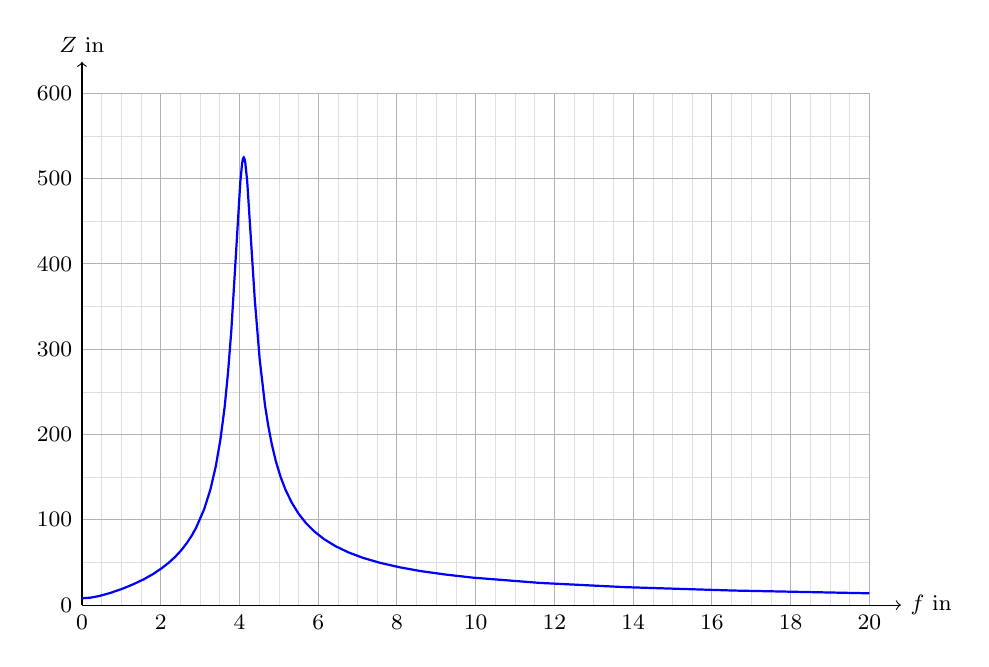
\begin{tikzpicture}[font=\footnotesize]
 \draw[gray!25, very thin] (0.250,0) -- (0.250,6.500) (0.500,0) -- (0.500,6.500) (0.750,0) -- (0.750,6.500) (1.250,0) -- (1.250,6.500) (1.500,0) -- (1.500,6.500) (1.750,0) -- (1.750,6.500) (2.250,0) -- (2.250,6.500) (2.500,0) -- (2.500,6.500) (2.750,0) -- (2.750,6.500) (3.250,0) -- (3.250,6.500) (3.500,0) -- (3.500,6.500) (3.750,0) -- (3.750,6.500) (4.250,0) -- (4.250,6.500) (4.500,0) -- (4.500,6.500) (4.750,0) -- (4.750,6.500) (5.250,0) -- (5.250,6.500) (5.500,0) -- (5.500,6.500) (5.750,0) -- (5.750,6.500) (6.250,0) -- (6.250,6.500) (6.500,0) -- (6.500,6.500) (6.750,0) -- (6.750,6.500) (7.250,0) -- (7.250,6.500) (7.500,0) -- (7.500,6.500) (7.750,0) -- (7.750,6.500) (8.250,0) -- (8.250,6.500) (8.500,0) -- (8.500,6.500) (8.750,0) -- (8.750,6.500) (9.250,0) -- (9.250,6.500) (9.500,0) -- (9.500,6.500) (9.750,0) -- (9.750,6.500);
 \draw[gray!25, very thin] (0,0.542) -- (10.000,0.542) (0,1.625) -- (10.000,1.625) (0,2.708) -- (10.000,2.708) (0,3.792) -- (10.000,3.792) (0,4.875) -- (10.000,4.875) (0,5.958) -- (10.000,5.958);
 \draw[gray!60, thin] (0.000,0) -- (0.000,6.500) (1.000,0) -- (1.000,6.500) (2.000,0) -- (2.000,6.500) (3.000,0) -- (3.000,6.500) (4.000,0) -- (4.000,6.500) (5.000,0) -- (5.000,6.500) (6.000,0) -- (6.000,6.500) (7.000,0) -- (7.000,6.500) (8.000,0) -- (8.000,6.500) (9.000,0) -- (9.000,6.500) (10.000,0) -- (10.000,6.500);
 \draw[gray!60, thin] (0,0.000) -- (10.000,0.000) (0,1.083) -- (10.000,1.083) (0,2.167) -- (10.000,2.167) (0,3.250) -- (10.000,3.250) (0,4.333) -- (10.000,4.333) (0,5.417) -- (10.000,5.417) (0,6.500) -- (10.000,6.500);
 \node[below] at (0.000,0) {0};
 \node[below] at (1.000,0) {2};
 \node[below] at (2.000,0) {4};
 \node[below] at (3.000,0) {6};
 \node[below] at (4.000,0) {8};
 \node[below] at (5.000,0) {10};
 \node[below] at (6.000,0) {12};
 \node[below] at (7.000,0) {14};
 \node[below] at (8.000,0) {16};
 \node[below] at (9.000,0) {18};
 \node[below] at (10.000,0) {20};
 \node[left] at (0,0.000) {0};
 \node[left] at (0,1.083) {100};
 \node[left] at (0,2.167) {200};
 \node[left] at (0,3.250) {300};
 \node[left] at (0,4.333) {400};
 \node[left] at (0,5.417) {500};
 \node[left] at (0,6.500) {600};
 \draw[->] (0,0) -- (10.400,0) node[right] {$f$ in \si{\kilo\hertz}};
 \draw[->] (0,0) -- (0,6.900) node[above] {$Z$ in \si{\kilo\ohm}};
 \draw[thick, blue] plot coordinates {(0.002,0.087) (0.103,0.094) (0.218,0.115) (0.358,0.154) (0.512,0.207) (0.655,0.266) (0.787,0.329) (0.907,0.397) (1.015,0.470) (1.105,0.541) (1.187,0.616) (1.262,0.698) (1.330,0.786) (1.394,0.882) (1.450,0.984) (1.552,1.218) (1.632,1.471) (1.700,1.765) (1.760,2.113) (1.812,2.514) (1.855,2.952) (1.897,3.488) (2.012,5.387) (2.034,5.610) (2.045,5.671) (2.055,5.685) (2.065,5.665) (2.075,5.612) (2.099,5.378) (2.195,3.879) (2.257,3.124) (2.325,2.536) (2.364,2.289) (2.407,2.061) (2.460,1.836) (2.520,1.636) (2.587,1.460) (2.664,1.302) (2.749,1.164) (2.845,1.041) (2.954,0.933) (3.076,0.837) (3.221,0.748) (3.386,0.669) (3.572,0.599) (3.786,0.537) (4.027,0.482) (4.301,0.432) (4.611,0.389) (4.962,0.349) (5.814,0.282) (6.899,0.228) (8.273,0.185) (10.000,0.150)};
\end{tikzpicture}
\end{center}

\begin{abcliste}
\abc At which frequency $f_0$ is the resonance peak?
\abc What is the capacitance $C$ of pickup and cable together?
\abc How long is the cable?
\end{abcliste}
